  % Custom margins for this section
\chapter{Fistful}
\noindent Karta udalosti sa odhaľuje od druhého ťahu šerifa ešte pred jeho vlastným ťahom a jej efekt platí, kým ju neprekryje ďalšia udalosť. Formulácia „na začiatku ťahu“ znamená ešte pred akoukoľvek inou akciou hráča.
\begin{figure}[!h]
    \centering
    \begin{minipage}[t]{\minipageSize}\centering
      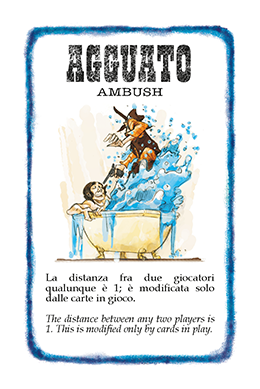
\includegraphics[width=\cardSize\linewidth]{fistful/05_agguato.png}
      \caption[Agguato]{Vzdialenosť medzi akýmikoľvek dvoma hráčmi je 1. Túto vzdialenosť menia iba karty v hre.}
    \end{minipage}
    \hfill
     \begin{minipage}[t]{\minipageSize}\centering
      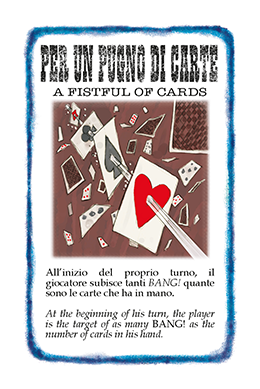
\includegraphics[width=\cardSize\linewidth]{fistful/05_perunpugnodicarte.png}
      \caption[Per un Pugno di Carte]{Na začiatku ťahu je na každého hráča vystrelených toľko BANG!-ov, koľko kariet drží v ruke.}
    \end{minipage}
    \hfill
     \begin{minipage}[t]{\minipageSize}\centering
      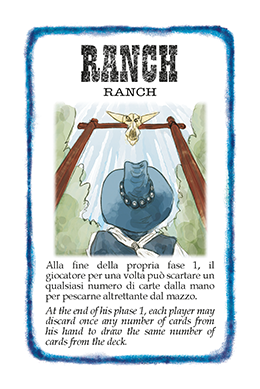
\includegraphics[width=\cardSize\linewidth]{fistful/05_ranch.png}
      \caption[Ranch]{Na konci fázy 1 môže hráč raz odhodiť ľubovoľný počet kariet z ruky a dobrať si za ne rovnaký počet nových.}
    \end{minipage}
    \hfill
    \begin{minipage}[t]{\minipageSize}\centering
      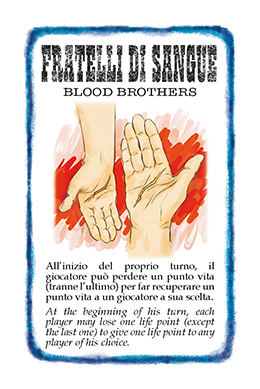
\includegraphics[width=\cardSize\linewidth]{fistful/05_fratellidisangue.png}
      \caption[Fratelli di Sangue]{Na začiatku ťahu môže hráč darovať jeden svoj život (okrem posledného) inému hráčovi podľa vlastného výberu.}
    \end{minipage}
\end{figure}

\begin{figure}[!h]
    \centering
    \begin{minipage}[t]{\minipageSize}\centering
      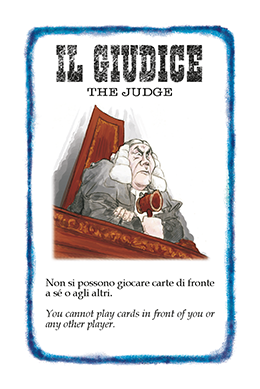
\includegraphics[width=\cardSize\linewidth]{fistful/05_ilgiudice.png}
      \caption[Il Giudice]{Nemôžete vyložiť karty pred seba alebo pred iných hráčov.}
    \end{minipage}
    \hfill
    \begin{minipage}[t]{\minipageSize}\centering
      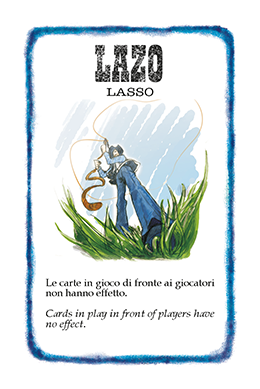
\includegraphics[width=\cardSize\linewidth]{fistful/05_lazo.png}
      \caption[Lazo]{Karty, ktoré sú vyložené pred hráčmi, neúčinkujú. Platí pre modré aj zelené karty.}
    \end{minipage}
    \hfill
    \begin{minipage}[t]{\minipageSize}\centering
      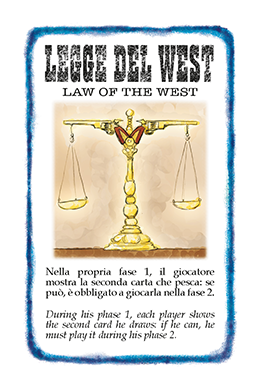
\includegraphics[width=\cardSize\linewidth]{fistful/05_leggedelwest.png}
      \caption[Legge del West]{Počas fázy 1 ukáže každý hráč druhú kartu, ktorú si doberá: ak môže, musí ju počas fázy 2 zahrať.}
    \end{minipage}
    \hfill
    \begin{minipage}[t]{\minipageSize}\centering
      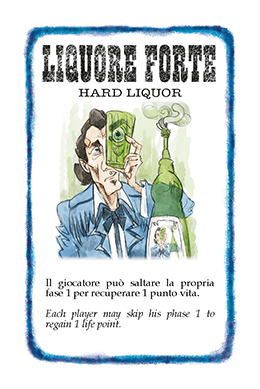
\includegraphics[width=\cardSize\linewidth]{fistful/05_liquoreforte.png}
      \caption[Liquore Forte]{Každý hráč môže preskočiť fázu 1 a získať tým 1 život.}
    \end{minipage}
\end{figure}

\begin{figure}[!h]
    \centering
    \begin{minipage}[t]{\minipageSize}\centering
      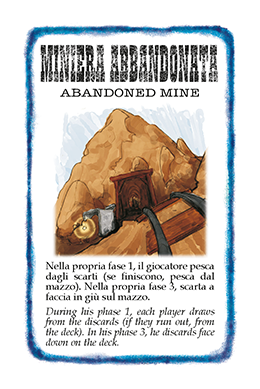
\includegraphics[width=\cardSize\linewidth]{fistful/05_minieraabbandonata.png}
      \caption[Miniera Abbandonata]{Počas fázy 1 si každý hráč berie karty z odhadzovacieho balíčka; ak je prázdny, berie ich z dobracieho balíčka. Počas fázy 3 sa karty odhadzujú lícom nadol na spodok dobracieho balíčka. Takto sa ukladajú iba karty, ktoré sa naozaj odhadzujú, napríklad vo fáze 3 alebo pri Dueli. Efekt vždy platí iba pre hráča, ktorý je práve na ťahu. Napríklad hráč, ktorý sa vyhol efektu Bang!, odhodí kartu Vedle! do bežnej odhadzovacej kopy. Efekt sa nevzťahuje na schopnosti postáv, napr. Jose Delgado. \cite{Fistful}}
    \end{minipage}
    \hfill
     \begin{minipage}[t]{\minipageSize}\centering
      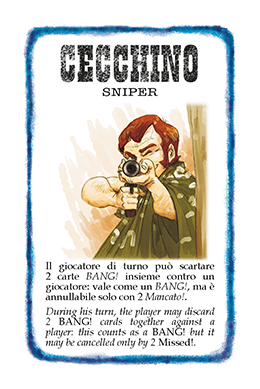
\includegraphics[width=\cardSize\linewidth]{fistful/05_cecchino.png}
      \caption[Cecchino]{Počas svojho ťahu môže hráč proti inému hráčovi odhodiť dve karty Bang! naraz. Stále ide len o jeden efekt Bang!, teda o stratu 1 života, ale odvrátiť ho možno iba dvoma efektmi Vedle!. Využitie tohto efektu sa nepočíta do limitu Bang!. \cite{Fistful}}
    \end{minipage}
    \hfill
    \begin{minipage}[t]{\minipageSize}\centering
      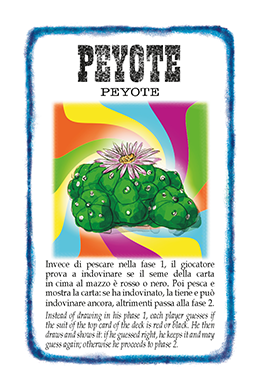
\includegraphics[width=\cardSize\linewidth]{fistful/05_peyote.png}
      \caption[Peyote]{Namiesto ťahania kariet vo fáze 1 tipuje každý hráč, či je karta na vrchu balíčka červená alebo čierna. Ak uhádne, kartu si nechá a môže tipovať znova, inak pokračuje do fázy 2. Hráč si nenecháva ani neuhádnutú kartu. Teda je možné že vo fáze 1 nedostane žiadnu kartu. \cite{Fistful}}
    \end{minipage}
    \hfill
    \begin{minipage}[t]{\minipageSize}\centering
      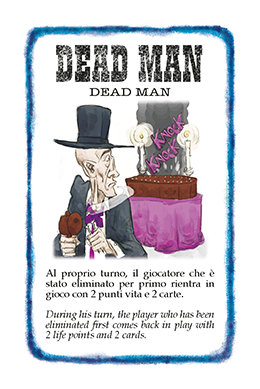
\includegraphics[width=\cardSize\linewidth]{fistful/05_deadman.png}
      \caption[Dead Man]{Hráč, ktorý vypadol ako prvý, sa počas svojho ťahu vracia do hry s 2 životmi a 2 kartami. Hráč si následne ťahá aj za fázu 1. Do hry sa môžte vrátiť aj keď ste zomreli pred vaším ťahom a Dead Man je práve v hre.}
    \end{minipage}
\end{figure}

\begin{figure}[!h]
    \centering
    \begin{minipage}[t]{\minipageSize}\centering
      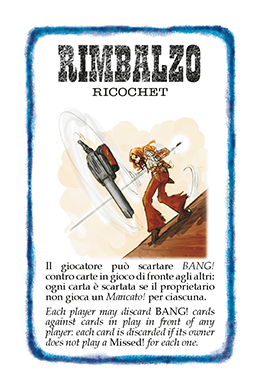
\includegraphics[width=\cardSize\linewidth]{fistful/05_rimbalzo.png}
      \caption[Rimbalzo]{Každý hráč môže odhodiť kartu BANG! proti karte vyloženej pred akýmkoľvek hráčom: ak hráč nepoužije efekt Vedľa!, zasiahnutá karta sa odhodí. Dostrel nie je potrebný pri využití tohto efektu. \cite{Fistful}}
    \end{minipage}
    \hfill
    \begin{minipage}[t]{\minipageSize}\centering
      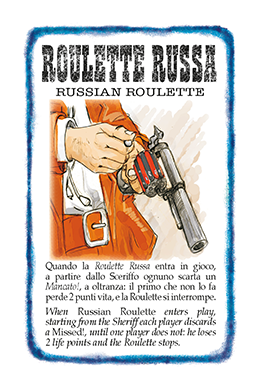
\includegraphics[width=\cardSize\linewidth]{fistful/05_rouletterussa.png}
      \caption[Roulette Russa]{Keď začne účinkovať Ruská ruleta, všetci hráči odhadzujú karty s efektom Vedľa! až kým jeden z nich nemá čo odhodiť: ten stratí 2 životy a ruleta končí.}
    \end{minipage}
    \hfill
    \begin{minipage}[t]{\minipageSize}\centering
      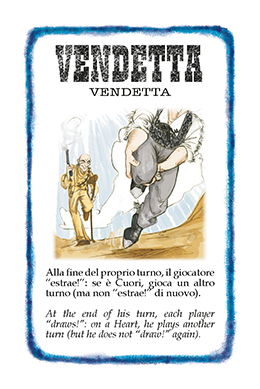
\includegraphics[width=\cardSize\linewidth]{fistful/05_vendetta.png}
      \caption[Vendetta]{Na konci ťahu každý hráč „sejme“: ak je karta srdcová, hrá ešte raz (ale už znovu „nesejme“).}
    \end{minipage}
       \hfill
    \begin{minipage}[t]{\minipageSize}\centering
    \end{minipage}
\end{figure}
